\documentclass[letterpaper,10pt]{article}
\usepackage{graphicx}
% \usepackage{osameet2}
\usepackage{amsmath,amssymb}


\begin{document}
\title{Automated Design of Nanophotonic Waveguide Couplers}
\author{Jesse Lu and Jelena Vu\v{c}kovi\'{c}}
% \address{Stanford University, Stanford, California, USA.}
% \email{jesselu@stanford.edu}

\maketitle
\begin{abstract}
We demonstrate a design algorithm which automatically generates 
    wavelength-scale coupling devices between arbitrary waveguide modes 
    with high efficiency.
Our algorithm is computationally fast, 
    can be extended to multiple dimensions,
    and requires no trial-and-error.
\end{abstract}
% \ocis{230.7370, 130.3990.}

% \begin{thebibliography}{99}
% \bibitem{lipson} Almeida et al, Optics Letters \textbf{28}, 1302-1304 (2003).
% \end{thebibliography}
% Importance of problem.

\section{Motivation}

% Why is waveguide mode conversion important?
\subsection{The importance of waveguide mode conversion}
Optical mode conversion, 
    the efficient transfer of photons from one guided mode to another,
    is a fundamental requirement in nanophotonics.
Efficient conversion between waveguides modes
    is critical in the many cases, including:
\begin{enumerate}
    \item Coupling to and from optical fiber\cite{}, 
        to communicate with the outside world.
    \item Coupling between various nanophotonic waveguides, 
        since different waveguides are best suited for different applications.
        For example, ridge waveguides seem ideal for low-loss transport\cite{},
            but other waveguides, 
            such as photonic crystal waveguides or slot waveguides,
            may be better suited for slow-light\cite{} 
            or energy-focusing devices\cite{}.
    \item Coupling between different materials.
       This is to couple between passive, active\cite{}, 
        and non-linear\cite{} materials. 
\end{enumerate}

% Why are current solutions insufficient?
\subsection{Common approaches to designing waveguide couplers}
% Brute force
Brute-force parameter search is the most popular nanophotonic design strategy 
    to-date because of its sheer simplicity\cite{}.
Although it may be suitable for tuning existing designs\cite{},
    the parameter space for most practical devices is simply too large
    for such a strategy to be tractable.

% Adiabatic mode conversion (large devices, symmetry breaking)
Adiabtic mode conversion strategies have been succesful
    for certain fiber-waveguide\cite{} and waveguide-waveguide\cite{} couplers,
    although resulting devices are quite large.
However, adiabatic strategy cannot be used in many important cases such as
    coupling from ridge to some photonic crystal waveguides,
    coupling in the out-of-plane direction, and
    coupling between modes of opposite symmetry.

% Local optimization
Optimization methods based on local derivatives seem very promising\cite{},
    in that they are both much faster than brute-force methods and
    more adaptable than adiabatic strategies.
However, these methods still require that every updated design be simulated
    at least once,
    and for the user to supply an initial design.


% How does your algorithm solve this problem?
\subsection{Advantages of objective-first design}
We present an ``objective-first'' approach to nanophotonic design, 
    and apply it to the problem of high-efficiency waveguide couplers.
The resulting algorithm
\begin{itemize}
    \item does not employ brute-force parameter searches,
    \item does not require a good initial design,
    \item is computationally fast (no simulations required),
    \item generates couplers between seemingly arbitrary waveguide modes, and
    \item can generate these couplers in a very small footprint. 
\end{itemize}

\section{Methods}
% What is objective-first optimization?
\subsection{Objective-first optimization}
The typical approach to designing physical structures can be formulated 
    in the following way, 
    where $x$ is the field variable and $p$ is the structure variable,
    \begin{subequations}\label{eq:adj}
    \begin{align} 
    \text{decrease} & \quad f(x) \label{eq:adj:obj} \\ 
    \text{subject to} & \quad g(x,p) = 0. \label{eq:adj:con}
    \end{align}
    \end{subequations}
Here, $f(x)$, the \emph{design objective}, 
    calculates the performance of the device 
    (e.g. amount of power not coupled to output mode); 
    while $g(x,p)$ is the underlying physical equation for the system
    (e.g. the electromagnetic wave equation).

In contrast, the objective-first formulation is
    \begin{subequations}\label{eq:ob1}
    \begin{align} 
    \text{decrease} & \quad \|g(x,p)\|^2 \label{eq:ob1:obj} \\ 
    \text{subject to} & \quad f(x) = 0, \label{eq:ob1:con}
    \end{align}
    \end{subequations}
    where $\|g(x,p)\|^2$ is the \emph{physics residual}.
We term this formulation ``objective-first''
    because the design objective is prioritized even above satisfying physics;
    specifically, we force our design to always exhibit the desired performance
    ($f(x) = 0$).

The differences between Eqs.~\ref{eq:adj} and \ref{eq:ob1} are
\begin{enumerate}
    \item in Eq.~\ref{eq:adj}, we attempt to decrease the design objective 
            (Eq.~\ref{eq:adj:obj}), 
        while in Eq.~\ref{eq:ob1}, the design objective is kept at zero 
            (Eq.~\ref{eq:ob1:con}); 
    \item in Eq.~\ref{eq:adj}, we always satisfy the underlying physics 
            (Eq.~\ref{eq:adj:con}),
        while in Eq.~\ref{eq:ob1}, physics is not satisfied,
            since the physics residual is generally non-zero
            (Eq.~\ref{eq:ob1:obj}).
\end{enumerate}

Thus, the fundamental innovation in the objective-first approach
    is simply this:
    we forcibly impose the desired performance on the device at the expense of
    breaking the physics which govern its operation.

% What are the implications of the objective-first approach?
\subsection{Numerical implications of the objective-first approach}

While the differences between the design strategies presented in 
    Eqs.~\ref{eq:adj} and \ref{eq:ob1} are straightforward,
    the numerical implications are more subtle.

The first practical implication of the objective-first approach 
    is that the number of independent variables is increased to include
    both $x$ and $p$.
In Eq.~\ref{eq:adj}, the constraint that physics must be satisfied, $g(x,p)=0$, 
    essentially forces $x$ to be dependent on $p$,
    since the choice of $p$ implicitly determines the value of $x$
    (there is generally a one-to-one mapping from $p$ to $x$).
In contrast, Eq.~\ref{eq:ob1} allows both $x$ and $p$ to vary independently,
    because the constraint, $f(x)=0$, is only a function of $x$.

Secondly, the amount of computation needed to enforce the constraint is
    drastically reduced in the objective-first approach.
This is because Eq.~\ref{eq:adj} requires a full solution of $g(x,p)=0$
    (i.e. a full simulation of the structure, $p$) to compute $x$.
In contrast, the constraint $f(x)=0$ in Eq.~\ref{eq:ob1} 
    can often be enforced so quickly (as shown below) that 
    future implementations may even produce designs in the same amount of time
    as required to simulate them!

Lastly, the objective-first approach eliminates the need for even a reasonable
    initial design.
Generally, methods based on Eq.~\ref{eq:adj} require an initial design which
    already provides some limited functionality
    (e.g. a coupler which already transfers 
    a non-zero amount of power to the desired output mode).
In constrast, methods based on Eq.~\ref{eq:ob1} perform just as well
    when started from a completely non-functional design 
    (e.g. a coupler which transfers no power into the desired output mode).

Together, these implications result in a method
    that is computationally fast (since it does not require simulation), and
    that can be applied to non-intuitive problems 
    where a functional starting design is not readily available.

% How is it applied to waveguide coupler design?
\subsection{Objective-first approach to waveguide coupler design}
We apply an objective-first approach to the problem of designing 
    two-dimensional nanophotonic waveguide couplers.

We choose to work in the two-dimensional transverse electric mode,
    which only couples $E_x$, $E_y$, and $H_z$ ($E_z, H_x, H_y = 0$),
    since it is most relevant for on-chip devices\cite{}.
We choose to use $H_z$ as the field variable, 
    and $\epsilon^{-1}$ (inverse of the permittivity) 
    as the structure variable.
This results in the following representation of the physics residual, 
    based on the time-harmonic electromagnetic wave equation without sources;
    \begin{equation}
    \|g(H_z, \epsilon^{-1})\|^2 = 
    \| \nabla \times \epsilon^{-1} \nabla \times H_z - \mu \omega^2 H_z \|^2,
    \end{equation}
    where $\omega$ is the angular frequency,
    and $\mu$ is the permeability of free-space.

For the design objective, we choose a boundary element formulation
    based on $H_z^\text{perfect}$,
    where $H_z^\text{perfect}$ is constructed 
    of the exact input and output waveguide modes at the input and output ports,
    repectively, and of zero-amplitude fields at the unused ports.
The actual form of the design objective is simply, 
    \begin{equation}
    f(H_z) = \begin{bmatrix}
        H_z - H_z^\text{perfect} \\
        \frac{\partial H_z}{\partial n} - 
            \frac{\partial H_z^\text{perfect}}{\partial n}
        \end{bmatrix}_\text{boundary}
        = 0.
    \end{equation}
That is to say,
    the values of $H_z$ and $\partial H_z / \partial n$
    (spatial derivative along normal direction)
    along the device boundary are forced to be 
    those of a device with perfect performance 
    (100\% coupling efficiency).
     
Such a design objective is both extremely simple and widely adaptable 
    to the design of nearly every kind of nanophotonic device.
Most importantly, it is trivial to enforce,
    requiring only that we overwrite boundary field values.
Although there is ambiguity in the relative phases of 
    the input and output boundary fields,
    our experience suggests that successful designs are possible for 
    arbitrary choice of relative phase.

Finally, in any objective-first approach,
    the physics residual is never guaranteed to decrease to zero.
Thus, it is entirely possible to never achieve 
    a physically realizable field, $H_z$.
In such cases, which are the norm rather than the exception,
    we find that a relatively small residual usually leads to
    fairly good, although imperfect, device performance.
    
\subsection{Numerical methods used to solve the objective-first design problem}
The design problem is now
    \begin{subequations}\label{eq:act}
    \begin{align} 
    \text{decrease} & \quad  
        \| \nabla \times \epsilon^{-1} \nabla \times H_z - \mu \omega^2 H_z \|^2
        \label{eq:act:obj} \\ 
    \text{subject to} & \quad 
        \left. H_z - H_z^\text{perfect} \right| _\text{boundary} = 0 
        \label{eq:act:con1} \\
        & \quad 
        \left. \frac{\partial H_z}{\partial n} - 
        \frac{\partial H_z^\text{perfect}}{\partial n} \right|_\text{boundary}
            = 0. \label{eq:act:con2}
    \end{align}
    \end{subequations}

This problem contains many local minima (it is non-convex\cite{});
    however, when either the field ($H_z$) or the structure ($\epsilon^{-1}$)
    variable is considered separately Eq.~\ref{eq:act} has only one minimum
    (it is convex), and can be easily solved using standard methods.
We employ such an alternating directions strategy,
    where both $H_z$ and $\epsilon^{-1}$ are solved independently.
This process is extremely inefficient,
    but is employed because the underlying numerical methods
    do not require any tuning.
We expect considerable improvements in computational efficiency
    when more sophisticated algorithms are applied,
    especially those which can update $H_z$ and $\epsilon^{-1}$ independently.
    
Lastly, we limit the allowable values of $\epsilon$ to be between
    the permittivity of vacuum and of silicon,
    \begin{equation}
    \epsilon_0 \le \epsilon \le \epsilon_\text{silicon}.
    \end{equation}
A completely binary structure would be preferred,
    $\epsilon = \{\epsilon_0, \epsilon_\text{silicon}\}$,
    and will be pursued in a future work.
That said, the final designs presented here 
    all have significant portions which are already binary.


\section{Results}
The method described above is applied to 
    the design of three different waveguide couplers
    as shown in Figs.~\ref{fig:fiber}, \ref{fig:mode} and \ref{fig:aircore}.




% Coupling efficiency
% Design time
% Size of the device
% Frequency
\begin{figure}[htbp]
    \centering
    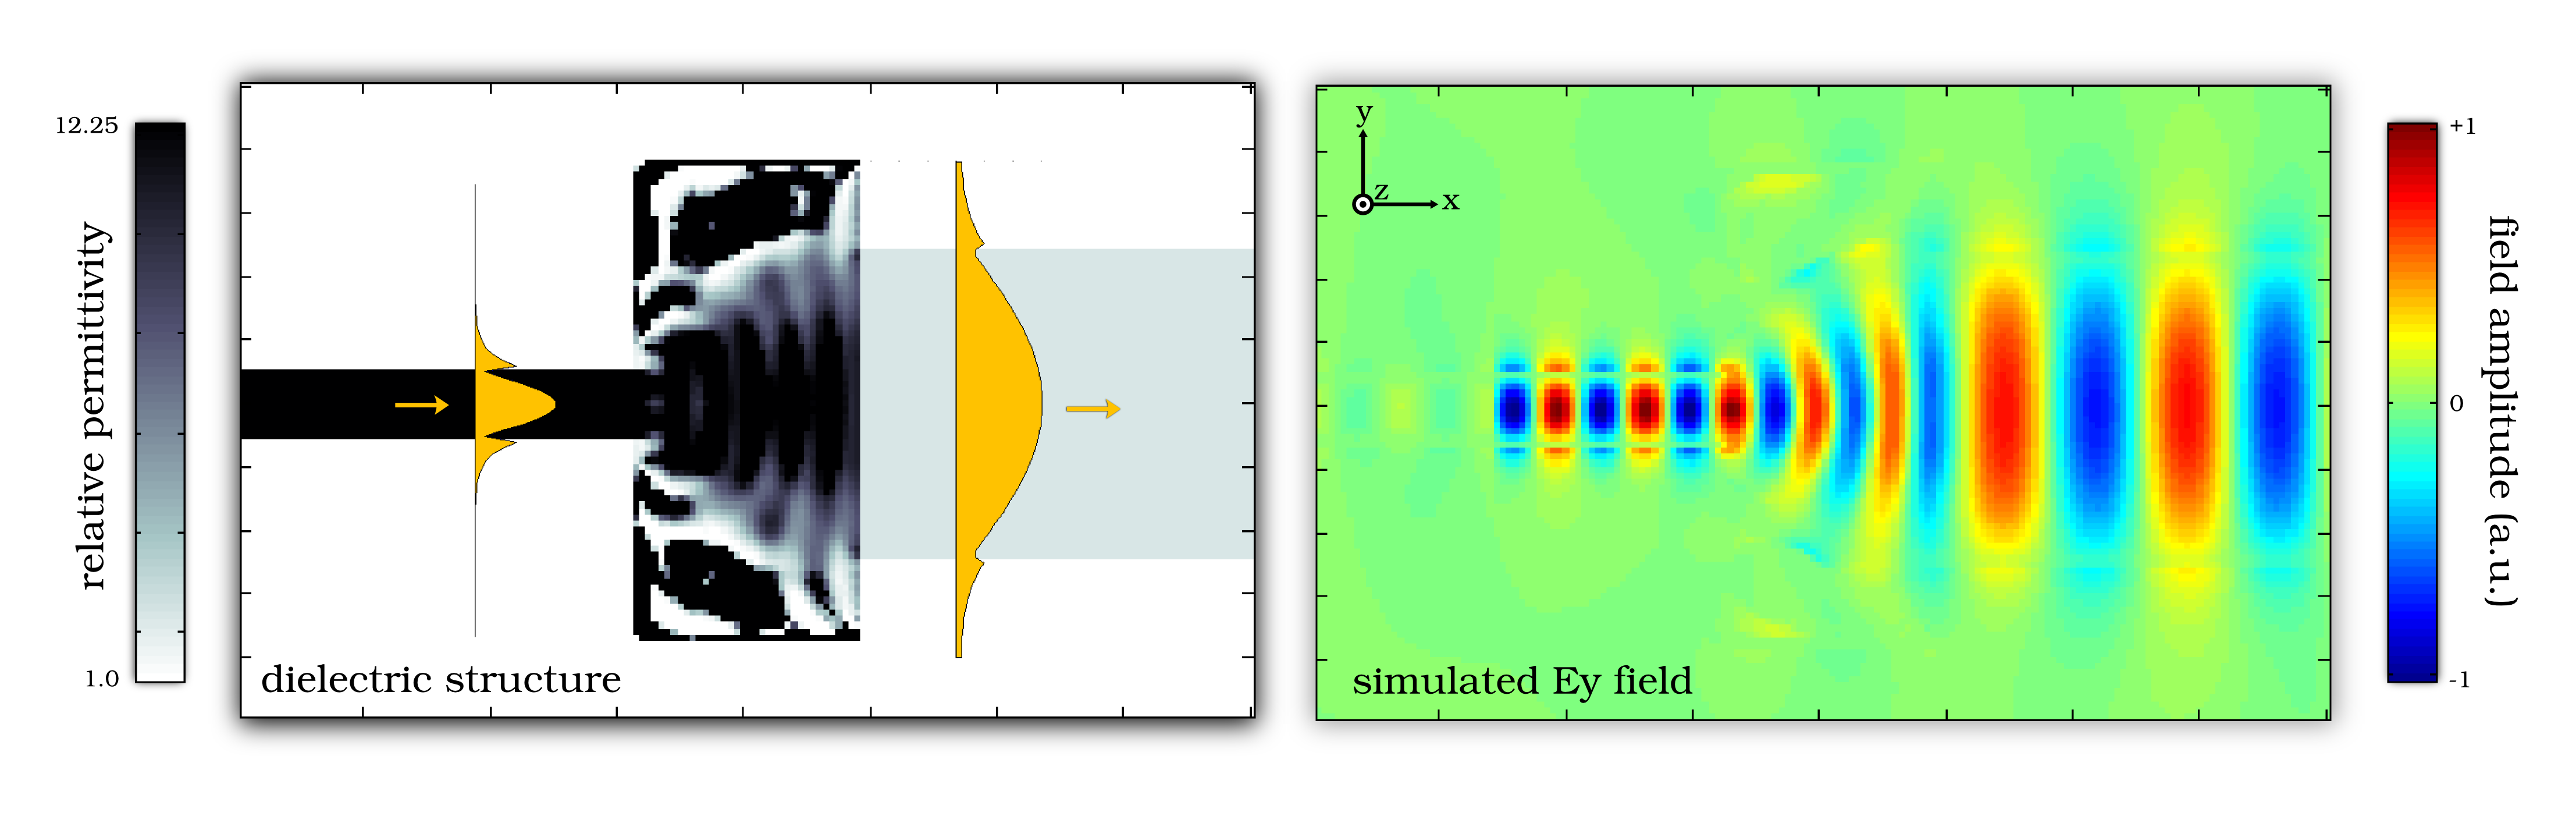
\includegraphics[width=\textwidth]{fig/fiber} 
    \caption{Waveguide coupler for a wide, low-index waveguide. 
        The dielectric structure of the coupler and surrounding input and
        output waveguides is shown on the left, while the simulation
        validating our results is shown on the right.
        The coupler converts $96.3\%$ of the input power to the
        designated output mode.
        The device is extremely compact, 
        convering only $36 \times 66$ grid points,
        where the vacuum wavelength is 42 grid points.
        Computation time was 20 minutes on a personal computer.}
    \label{fig:fiber}
\end{figure}
\begin{figure}[htbp]
    \centering
    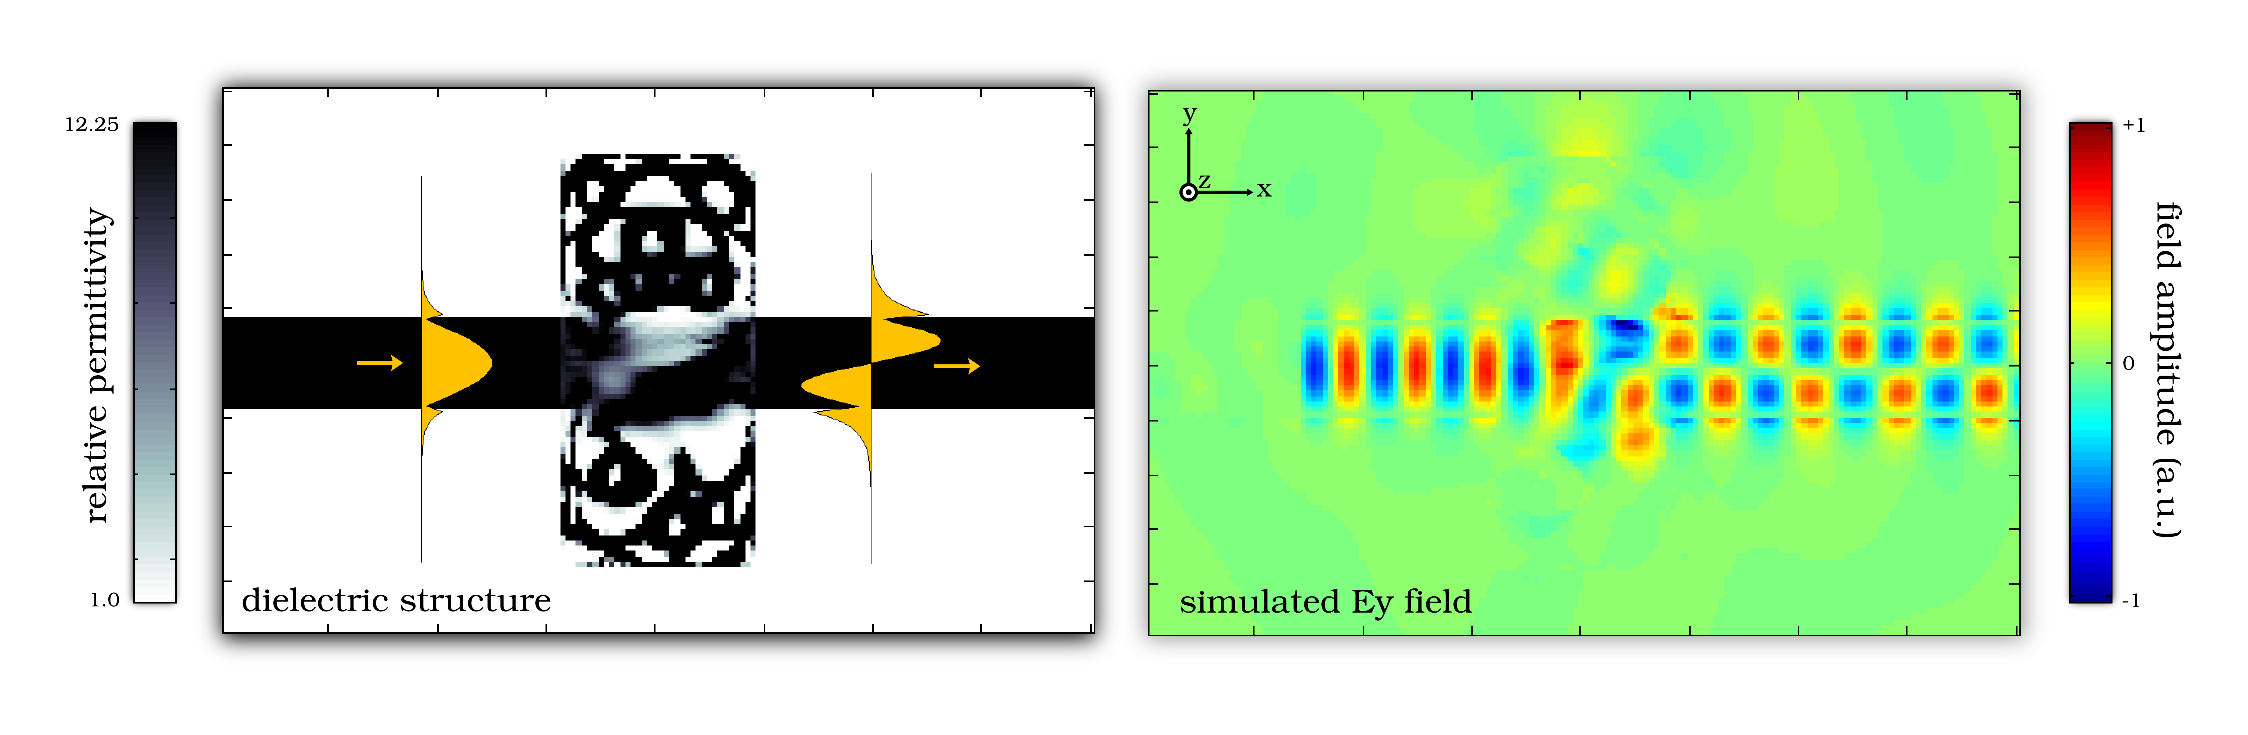
\includegraphics[width=\textwidth]{fig/mode-conv} 
    \caption{Coupler that converts the fundamental waveguide mode to the
        second-order waveguide mode.
        This problem is quite difficult since the two modes are of 
        opposite symmetry.
        For example, adiabatic approaches cannot be applied to this case.
        However, our method produces a device 
        (which has the same dimensions and vacuum wavelength as Fig. 1) 
        which achieves a coupling efficiency of $95.5\%$. 
        Computation time was extended to 50 minutes to improve efficiency.
        }
    \label{fig:mode}
    \end{figure}
\begin{figure}[htbp]
    \centering
    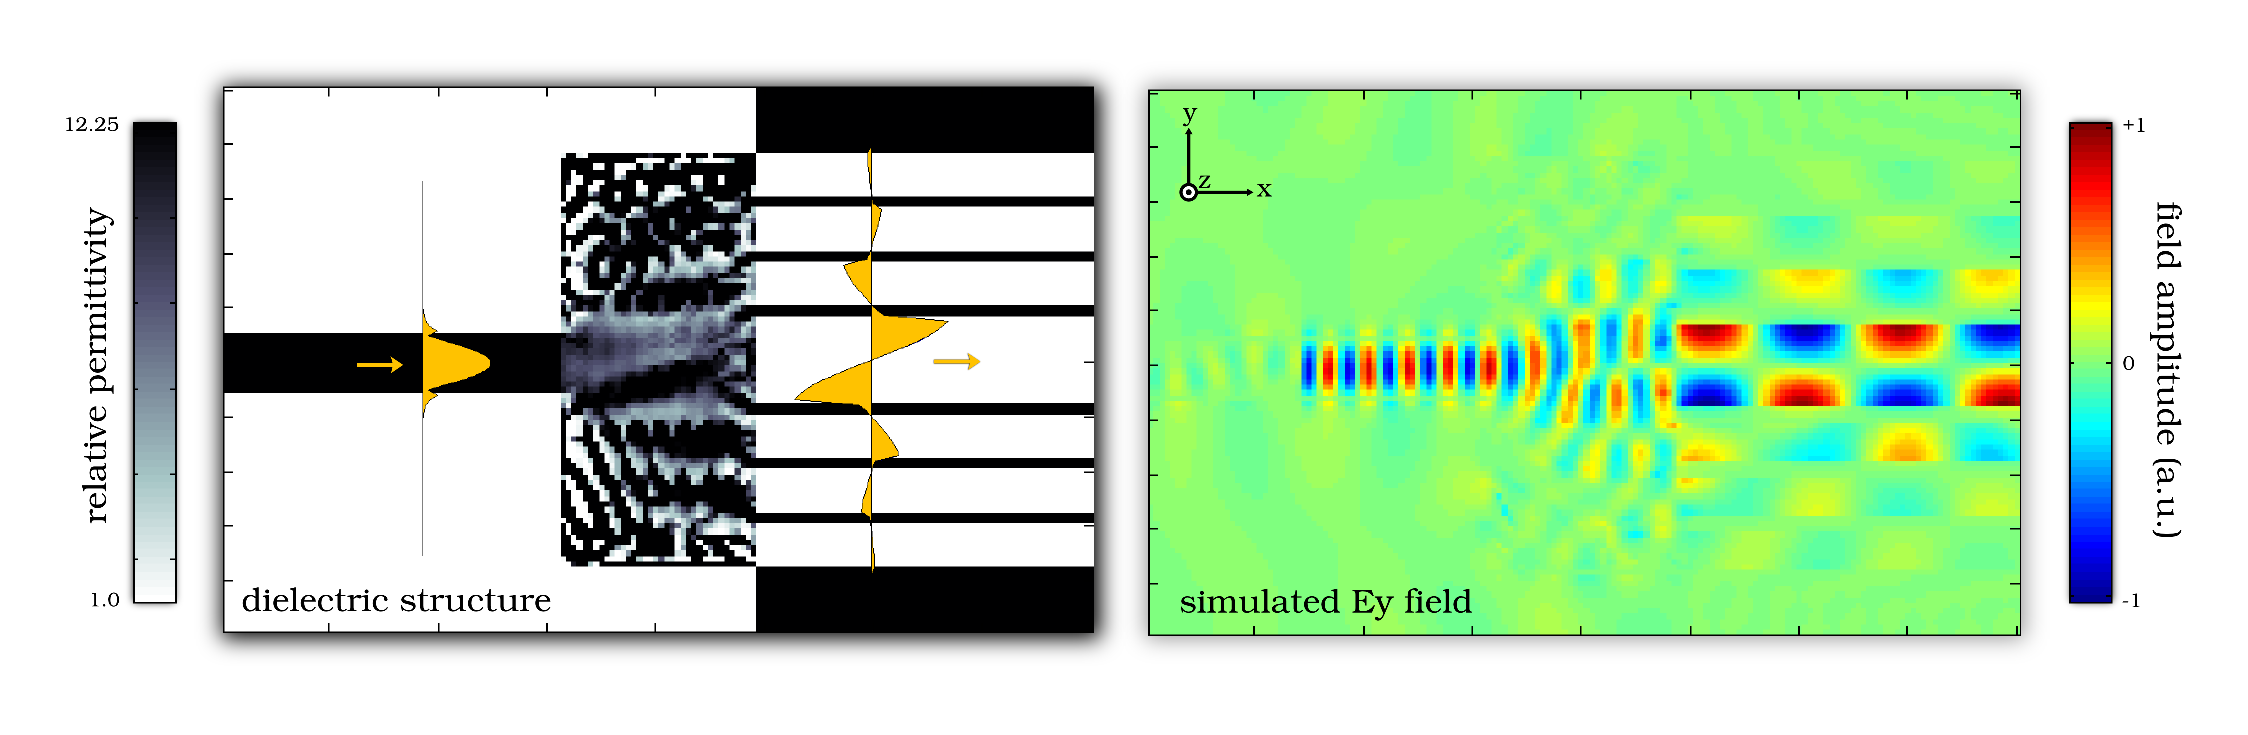
\includegraphics[width=\textwidth]{fig/air-core}
    \caption{Coupler to an air-core mode.
        Here, not only are the modes of opposite symmetry,
        but the output waveguide operates on a fundamentally different
        principle (guided by Bragg reflection) than the input waveguide 
        (index guided).
        The device still achieves an efficiency of $83.3\%$, demonstrating the
        versatility of our method.
        The vacuum wavelength is 25 grid points, 
        while the device footprint is still $36 \times 66$ grid points.
        Computation time was 20 minutes.
        }
        \label{fig:aircore}
\end{figure}

This work has been supported in part by the 
    AFOSR MURI for Complex and Robust On-chip Nanophotonics 
    (Dr. Gernot Pomrenke), grant number FA9550-09-1-0704.

\end{document}

